\chapter{Testing and Evaluation}
\label{cha:testing}

\begin{comment}
Chapter 6: Testing and Evaluation
This chapter should give details of how the system designed and implemented by you was tested. The data and results obtained from this testing whould be presented and consideration be given as to whether or not these results confirm that everything works correctly.

The analysis of test results is very important and some assessment of their significance and quality must be given. Likely sources of error and inaccuracy should be mentioned. Use graphs, bar charts and histograms where appropriate, remembering to label all axes and give scales. The analysis is often done badly, thus sacrificing marks.
\end{comment}

The evaluation of the application indicates that these three objectives have been met. Preliminary research demonstrates that enjoyed using the application and that the majority of participants would use it in the future if implemented as a full product. Testing with participant data shows that the average absolute error of the prediction engine was $PERCENTAGE\%$ for users with over three months historical information. Preliminary penetration testing, using both white-box and black-box testing indicated that the security protections put in place are effective.  However, the evaluation of the project was limited, due to the size of the user base, discussed further in \autoref{sec:limitations}. \todo{Complete this}

\section{During Development}
Though-out the development of the project, predominantly after each feature was implemented and before a new iteration was started the applications functionality was tested through face to face conversations, observations and unit testing.

\subsection{Acceptance Testing}
As noted throughout the report, the application was regularly tested by potential end users and the developers during lab observations where the user was asked to complete a task on the website while describing what they were doing. 

During the testing, common pain points were identified and these were used to decide on the future features, either to improve the user experience on the website, making it easier to use, or to support a new use case.

Example modifications, made as a result of these observations, include the dropdown menu autocompletion when creating and mapping transactors, the hints that appear throughout the website to guide the user onto the next task, and the suggestion wizard.

Towards the beginning of the project these meetings were used to evaluate and update the design of the user interface, which went through several different designs, and to receive qualitative feedback from the users (Fig. \ref{fig:ui-design}).

\begin{figure}
\centering
\begin{subfigure}{0.34\textwidth}
  \centering
  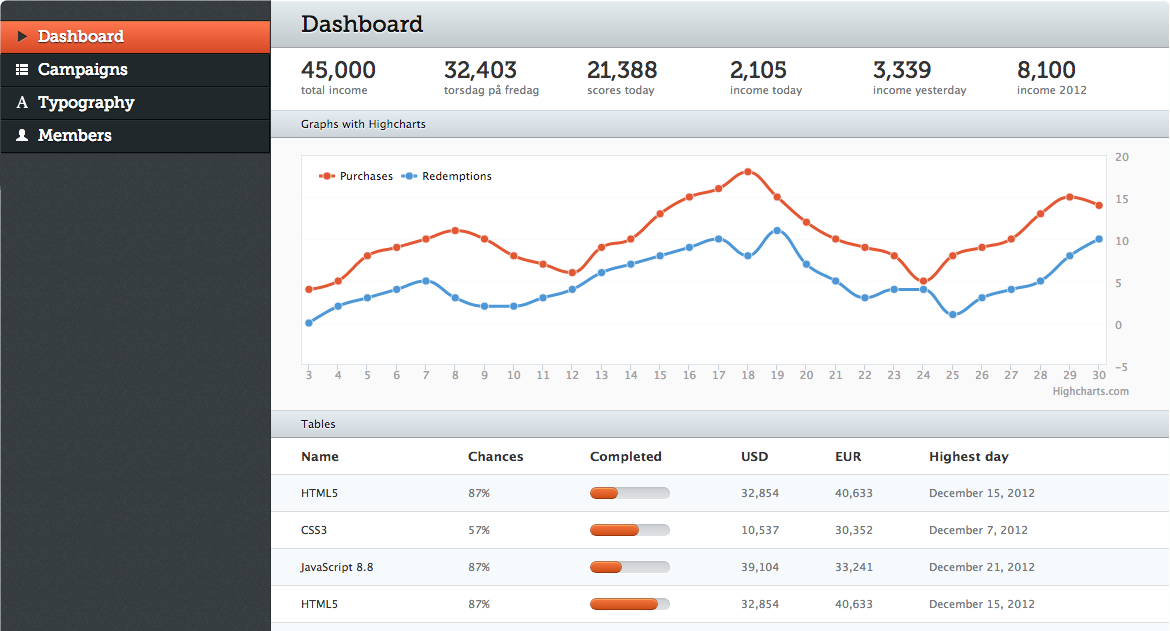
\includegraphics[width=0.95\linewidth]{testing/uidesign1}
\end{subfigure}%
\begin{subfigure}{0.34\textwidth}
  \centering
  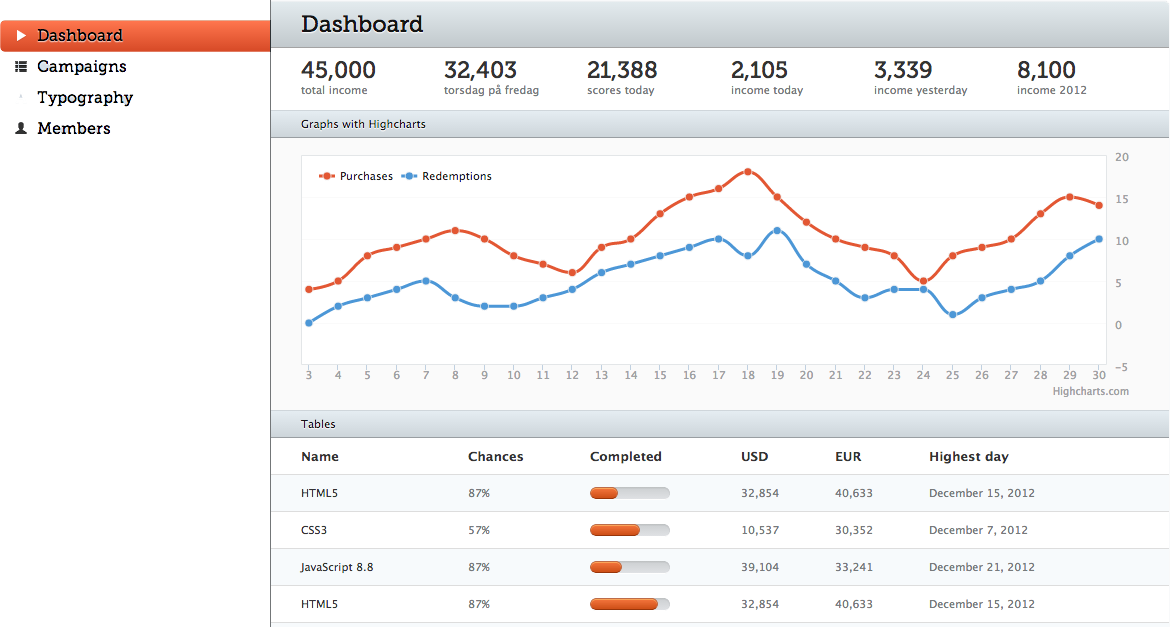
\includegraphics[width=0.95\linewidth]{testing/uidesign2}
\end{subfigure}
\begin{subfigure}{0.31\textwidth}
  \centering
  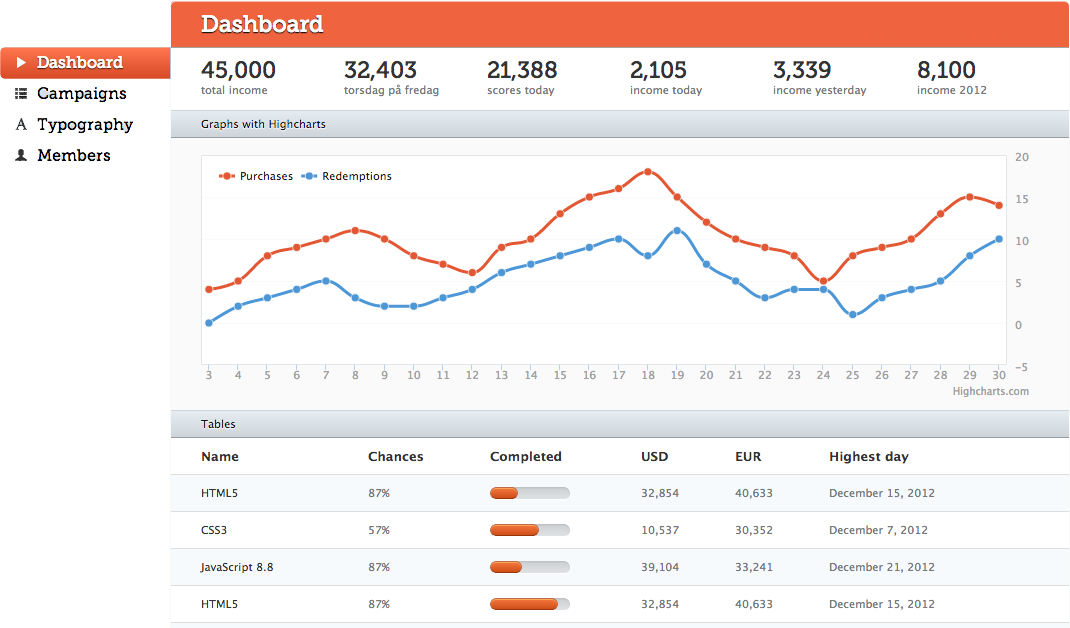
\includegraphics[width=0.95\linewidth]{testing/uidesign3}
\end{subfigure}
\caption{A few iterations of the user interface designs}
\label{fig:ui-design}
\end{figure}

\subsection{Unit Testing}
High risk classes, including the Budget, the QIF and OFX Parsers implementing the TransactionFileParserInterface, and those implementing the TransactionCollectionInterface were unit tested to ensure the functionality of the classes was not affected when implementing new features or refactoring the code.

These classes were selected as the core functionality of the application relied on their behaviour and they were coupled to the most other classes, for example the Budget object was responsible for holding a collection of Transactons in the tree data structure described in \autoref{section:prediction-implementation} and performed the majority of the prediction functionality, holding references to the TransactionMarkovChain, TransactionWeightedAverageCalculator and PredictionEvaluation.

Due to time constraints and the complications of testing data driven classes, both the number of unit tested classes and methods covered was limited, this is discussed further in \autoref{sec:limitations}.

\section{After Development}
Once development of the project was halted the application was tested in the three following the three sections outlined through the report. The statement management functionality was assessed using a questionnaire posed to research participants that were given access to the system, the prediction algorithms were evaluated using the sample data provided by the research participants and the security of the application was evaluated using penetration testing.
%
Unfortunately the reliability of the results for both the statement management and prediction is questionable due to the limited number of research participants and questionnaire responses, see \autoref{sec:limitations}.

% This chapter should give details of how the system designed and implemented by you was tested. The data and results obtained from this testing whould be presented and consideration be given as to whether or not these results confirm that everything works correctly.
% The analysis of test results is very important and some assessment of their significance and quality must be given. Likely sources of error and inaccuracy should be mentioned. Use graphs, bar charts and histograms where appropriate, remembering to label all axes and give scales. The analysis is often done badly, thus sacrificing marks.

\subsection{Statement Management}
The questionnaire posed to the research participants was split into three sections, a full copy of the questions can be found in Appendix \ref{app:questionnaire}.

The first made a series of statements and asked the respondent to answer on a five point scale, ranging from 1, strongly disagree to 5, strongly agree. The questions in this section had four main types, and were selected following the structure of the Standardized Universal Percentile Rank-Questionnaire which is used by companies including PayPal to assess their websites \parencite{sauro2011standardized}. 
%
Questions on usability focused on how easy users found navigation of the website, locating the information they needed, and whether they enjoyed using it.
%
The potential loyalty of the participants was judged by using the likely hood of a user recommending the site to their colleagues and friends or returning to the site in the future.

The second section focused on task completion, participants were asked to complete a task and then rate the how difficult or easy they found that on a seven point scale.
%
This section was designed to assess the functionality of the website and to identify additional pain points.
%
One scale question was asked per task as research suggests that use of a single question performs just as well as breaking the task down into sub-questions \parencite{sauro2009comparison, sauro2009correlations}, however a free text field was included with each task to obtain qualitative information on the reasons behind the answer.

In final section was used to identify features of the the website that users favoured and those they disliked in order to backup the points reviewed in section two, all questions were answered in free text fields.

In the first section, answered on a 1-5 scale, Loyalty was the question type with the highest average score of 4.10 and a standard deviation of 1.66, which indites some uncertainly, further analysis of the answers, shown in Fig. \ref{fig:box-loyalty}, shows that the majority of answers fell between the first and third quartiles and that the median value was 5, indicating that the result is being negatively skewed and affected by outliers at the low end.
%
The statement with the highest average level of agreement was `If completed, I would visit this site in the future' with an average answer of 4.20, though the standard deviation again quite high at 1.79. Hopefully, this implies that the automation of budget management was of useful to the majority of participants and has potential as a real world product.
%
The usability questions received the lowest score, with an average agreement of 3.50 which is slightly agree. The box plot for the usability questions is shown in Fig. \ref{fig:box-usablity} which indicates that the mean is a fair measure of this data, though the data is negatively skewed, it also shows that, although the median answer was 4.00 answers ranged between 1 and 5.
%
The questions with the lowest agreement level, overall, were both within usability. `The website is easy to use' and `I am able to find what I need quickly' which both scored 3.00, with a standard deviation of 1.41 and 1.22 respectively. On the scale a 3 is neutral, the respondents neither agree or disagree with the statement.
%
The relatively low agreement level of the usability questions was a surprise. It was believed that the hints shown throughout the site and the single navigation menu had improved the usability of the website, however it's clear this area may need extra work.

\begin{figure}
\centering
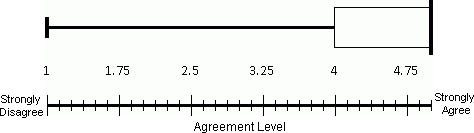
\includegraphics[width=0.75\textwidth]{testing/box-plot-loyalty}
\caption{Box plot of Loyalty question responses\protect\footnotemark}
\label{fig:box-loyalty}
\end{figure}

\footnotetext{The whiskers indicate the minimum and maximum values}

\begin{figure}
\centering
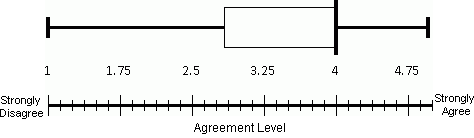
\includegraphics[width=0.75\textwidth]{testing/box-plot-usability}
\caption{Box plot of Loyalty question responses}
\label{fig:box-usablity}
\end{figure}

The responses to the task difficulty questions, shown in Fig. \ref{fig:box-difficulty}, indicated that the most difficult tasks to complete were downloading a the users statement from their online banking account and viewing their monthly predictions.
%
Downloading statements may be outside the control of the application, but comments including `difficult selecting the dates that you want' and `not sure which download option to choose' indicate that more detailed guidance could be provided to the users when they're told to download their statement.
%
The relatively low score of the monthly prediction section of the website, is supported with comments including `too much information' and `very messy screen', suggesting that further work should be done to improve it's layout and to reduce the amount of detail shown.
%
Overall the responses to the task difficulty questions are positive, with an average difficulty rating of 5.7, indicating that website is relatively easy to use.

The textual responses to the questions in the final section were in line with the task difficulty measures, with difficult tasks noted as the least useful. Interestingly, the pie chart breaking down the expenditure per category was selected as the most useful feature by 100\% of the respondents who answered the question, which was matches the background research for existing applications.

\begin{figure}
\centering
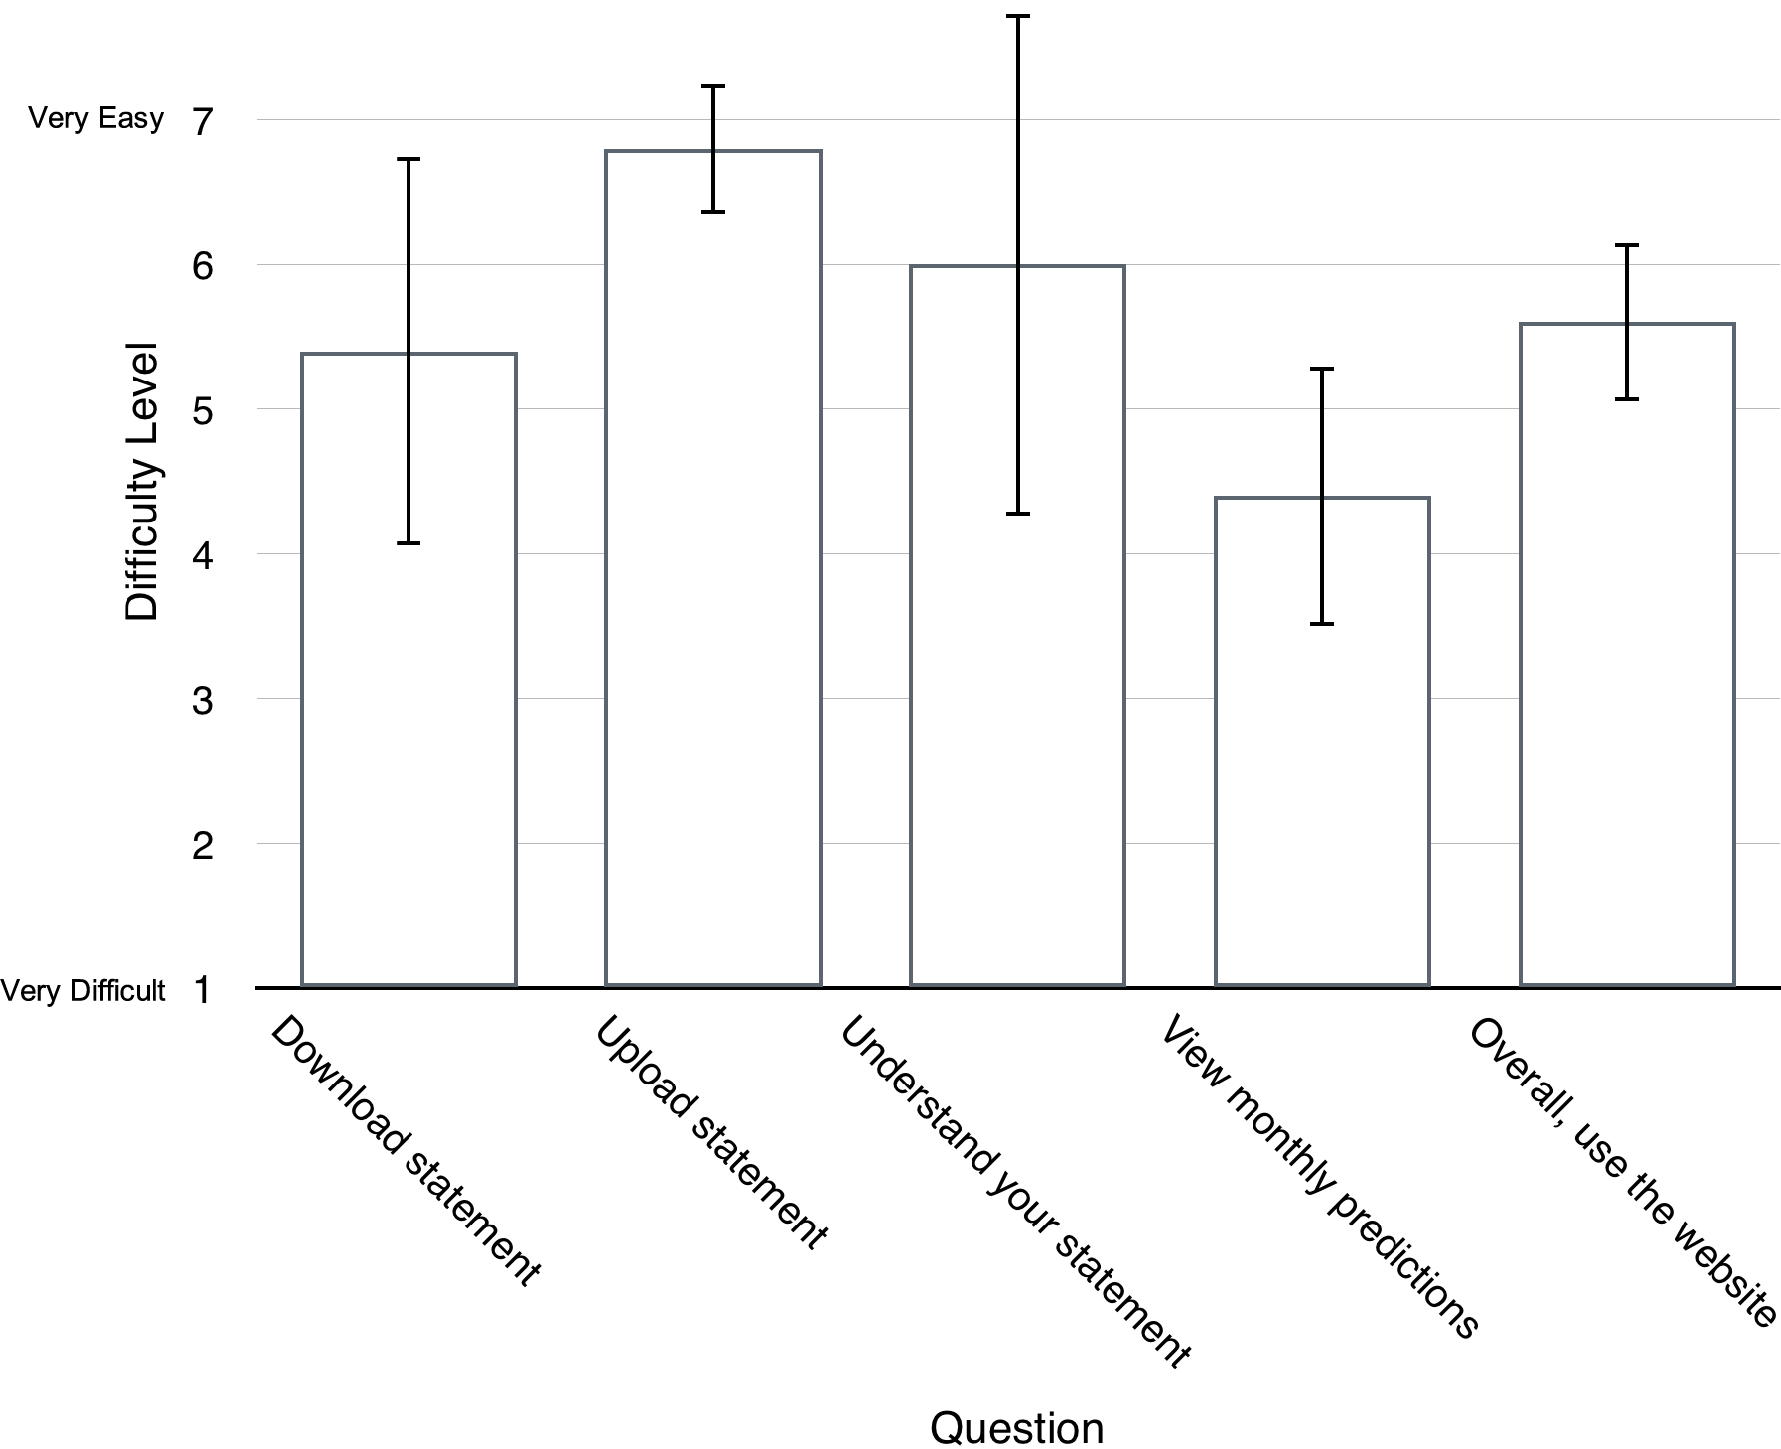
\includegraphics[width=0.75\textwidth]{testing/difficulty-bar}
\caption[Responses to the task difficulty questions]{Responses to the task difficulty questions, the standard deviation is shown as error bars}
\label{fig:box-difficulty}
\end{figure}

\subsection{Prediction}
By taking the test participant data, it was possible to evaluate the prediction accuracy of the application. Users with more than four months history were selected and the data was split into two halves. All but the most recent complete month was fed to the prediction engine and used to make a prediction for total spending and income in the known month. By comparing the recorded predictions to the actual values for that month it was possible to calculate the absolute and percentage error.

Overall the system performed with 16.7\% average error, performing with a lower average error of 14.6\% for income and a slightly higher error of 18.4\%. It is likely that income has a lower error as the income is often regular and for similar amounts.
%
However, as only 7 of the participants had uploaded more than four months data the scope of the testing was limited and the reliability of the results is questionable. In addition, three of the records were identified as outliers as the absolute error fell significantly outside of the inter quartile range, and not included in the averages. Outliers were identified using $\big[ Q_1 - 1.5 (Q_3 - Q_1) , Q_3 + 1.5 (Q_3 - Q_1) \big]$ where  $Q_1$ and $Q_3$ were the upper and lower quartiles. 
%
The full results of the testing data are shown in Table \ref{tab:rawtestingdata} and the quartiles are shown in Table \ref{tab:quartiles}, records that fell outside of the bounds and were ignored when calculating the averages are indicated in italics. 
%
It is likely that these outliers were caused by sudden changes in spending pattern or that the prediction is being affected by significant expenditure or income in January.

\begin{table}[h]
\centering
\begin{tabular}{@{}lllllll@{}}
\toprule
     &             &  \multicolumn{2}{c}{February} & & \\
User & Type        & Prediction (£) &  Actual (£) & Absolute Error (£)                      & Error (\%)               \\ \midrule
1    & Income      & 1620                & 1409            & 211                                  & 15.0           \\
     & Expenditure & 1710                & 2603            & 893                                  & 34.3           \\
2    & Income      & 2080                & 209             & 1871                                 & \textit{895.2} \\
     & Expenditure & 1678                & 1633            & 45                                   & 2.8            \\
3    & Income      & 1187                & 1200            & 13                                   & 1.1            \\
     & Expenditure & 1227                & 943             & 284                                  & 30.1           \\
4    & Income      & 864                 & 881             & 17                                   & 1.9            \\
     & Expenditure & 659                 & 814             & 155                                  & 19.0           \\
5    & Income      & 1060                & 732             & 328                                  & 44.8           \\
     & Expenditure & 1101                & 1309            & 208                                  & 15.9           \\
7    & Income      & 243                 & 100             & 143                                  & \textit{143.0} \\
     & Expenditure & 383                 & 51              & 332                                  & \textit{651.0} \\
8    & Income      & 1008                & 914             & 94                                   & 10.3           \\
     & Expenditure & 1113                & 1029            & 84                                   & 8.2            \\
     &             &                     &                 & \multicolumn{1}{r}{\textbf{Average}} & \textbf{13.7}
\end{tabular}
\caption{The results of the prediction evaluation test, which compared predictions and actual values }
\label{tab:rawtestingdata}
\end{table}

\begin{table}[h]
\centering
\begin{tabular}{lll}
                & Quartile & Bound  \\
Lower Bound     & 8.7      & -172.6 \\
Second Quartile & 17.5     &        \\
Upper Bound     & 111.5    & 265.8 
\end{tabular}
\caption{First, second and third quartiles for the prediction evaluation test}
\label{tab:quartiles}
\end{table}

\subsection{Security}
The security of the application was measured using white-box and black-box penetration testing.
%
The author, who had a working knowledge of the internals of the application and access to the source code, performed the white-box testing. They attempted to break into the account of someone using the website through the use of session hijacking outlined in \autoref{subsection:account-hijacking}, even after disabling the encryption of the users session by temporarily allowing allow cookies to be sent over HTTP, and gaining a copy of the cookie the account couldn't be accessed as the users session was invalidated once the session hijack was detected by the fingerprinting mechanism. Even after the headers of the target user were cloned, the users session ID didn't match the one found in the database and the session was once again invalidated.
%
Black-box penetration testing was performed by a peer of the author, who has experience in penetration testing. The unsucesfully tried SQL injection by modifying the parameters sent in the suggestion wizards AJAX requests before uploading a bank statement that contained cross site-scripting (XSS) code designed to steal the users cookie. The uploaded statement was parsed successfully and all of the XSS was escaped, preventing the code injection. Finally, the tester attempted to upload malicious files in an attempt to break the upload feature, in all cases the 
%
Although this demonstration isn't able to conclude that the application is secure and resilient to all attacks, it does demonstrate that more common attacks including those outlined in \autoref{sec:back-security} are prevented.
